\chapter{Pengembangan Dan Pengujian}

\par Pada Tugas Akhir ini, perangkat lunak yang dikembangan berupa sistem manajemen kompetisi, \textit{autograder} dan program antar muka pengguna.  Sistem manajemen kompetisi di\textit{deploy} pada komputer yang disediakan oleh juri dan bertindak sebagai \textit{server}. \textit{Autograder} dan program antar muka akan didistribusikan kepada peserta dan juri untuk dijalankan pada komputernya. Secara keseluruhan, perangkat lunak yang dikembangkan dinamakan \textit{UGrade}. Nama tersebut berasal dari kata \textit{you} dan \textit{grade}. Nama tersebut dipilih karena proses penilaian atau \textit{grading} dilakukan oleh masing-masing peserta.

\par Terdapat tiga program utama yang dikembangkan pada \textit{UGrade} yaitu: \textit{UGServer}, \textit{UGJob} dan \textit{UGDesktop}. \textit{UGServer} berfungsi sebagai sistem manajemen kompetisi yang bertindak sebagai server. \textit{UGJob} berfungsi sebagai \textit{worker} dari \textit{autograder}. \textit{UGDesktop} berfungsi sebagai antar muka antara pengguna dengan sistem \textit{online judge}. Selain tiga program utama tersebut, terdapat program lain yang digunakan untuk membantu proses pengembangan. Untuk melakukan \textit{sandboxing}, dikembangan program yang bernama \textit{UGSbox}. Selain itu, untuk memudahkan proses testing, dikembangankan program \textit{UGCtl} yang dapat digunakan sebagai antar muka pengguna dalam bentuk \textit{command-line}.

\section{\textit{UGServer} (Sistem Manajemen Kompetisi)}

\par \textit{UGServer} merupakan sistem manejem kompetisi yang berfungsi untuk mengatur keberjalanan kompetisi. \textit{UGServer} memberikan layanan kepada peserta dan juri untuk berinteraksi dengan kompetisi. Layanan yang diberikan oleh \textit{UGServer} antara lain:
\begin{enumerate}
  \item Otentikasi dan otorisasi pengguna.
  \item Pembuatan dan akses kompetisi.
  \item Pembuatan dan akses soal pada kompetisi.
  \item Pengiriman dan akses jawaban pada kompetisi.
\end{enumerate}

\par Sebenarnya masih banyak layanan lain yang harus diberikan oleh sistem manajemen kompetisi. Akan tetapi, Tugas Akhir ini lebih difokuskan untuk mengembangkan \textit{autograder} dibandingkan dengan sistem manajemen kompetisi. Hal ini dikarenakan tujuan dari Tugas Akhir ini lebih berfokus pada proses penilaian jawaban peserta. Oleh karena itu, fungsionalitas yang dipaparkan pada paragram di atas sudah cukup untuk memenuhi tujuan dari Tugas Akhir ini.

\par \textit{UGServer} dikembangkan dengan menggunakan \textit{framework django}. Pengembangan perangkat lunak berbasis \textit{web} dapat dengan cepat dan mudah dilakukan menggunakan \textit{framework django}. Selain itu, \textit{django} telah memberikan banyak fitur yang sangat membantu proses pengembangan perangkat lunak seperti otorisasi, otentikasi, dan \textit{ORM}. Terdapat beberapa alternatif lain yang dapat meningkatkan kinerja sistem manajemen kompetisi seperti menggunakan \textit{express} atau \textit{GO}. Kedua alternatif tersebut tidak digunakan karena membutuhkan waktu pengembangan yang lama dan tidak terlalu memberikan perunbahan yang signifikan. Oleh karena itu, \textit{Framework} \textit{django} dipilih untuk mengembangkan \textit{UGServer} karena mudah dan cepat untuk dikembangkan.

\par \textit{UGServer} memberikan \textit{API} yang dapat digunakan oleh pengguna. \textit{API} yang diberikan oleh \textit{UGServer} berupa \textit{GraphQL} yang berjalan di atas protokol \textit{HTTP}. \textit{GraphQL} digunakan karena mudah untuk diimplementasikan dan digunakan. \textit{UGDesktop} dan \textit{UGCtl} merupakan program antar muka pengguna yang menggunakan \textit{API} ini. Terdapat beberapa alternatif lain yang dapat digunakan untuk mengembangkan \textit{API} dari \textit{UGServer} seperti menggunakan arsitektur \textit{REST} atau menggunakan teknik seperti \textit{RPC}. Alternatif tersebut tidak digunakan karena lebih tidak fleksibel dan lebih sulit untuk diimplementasikan.

\begin{figure}[ht!]
    \centering
    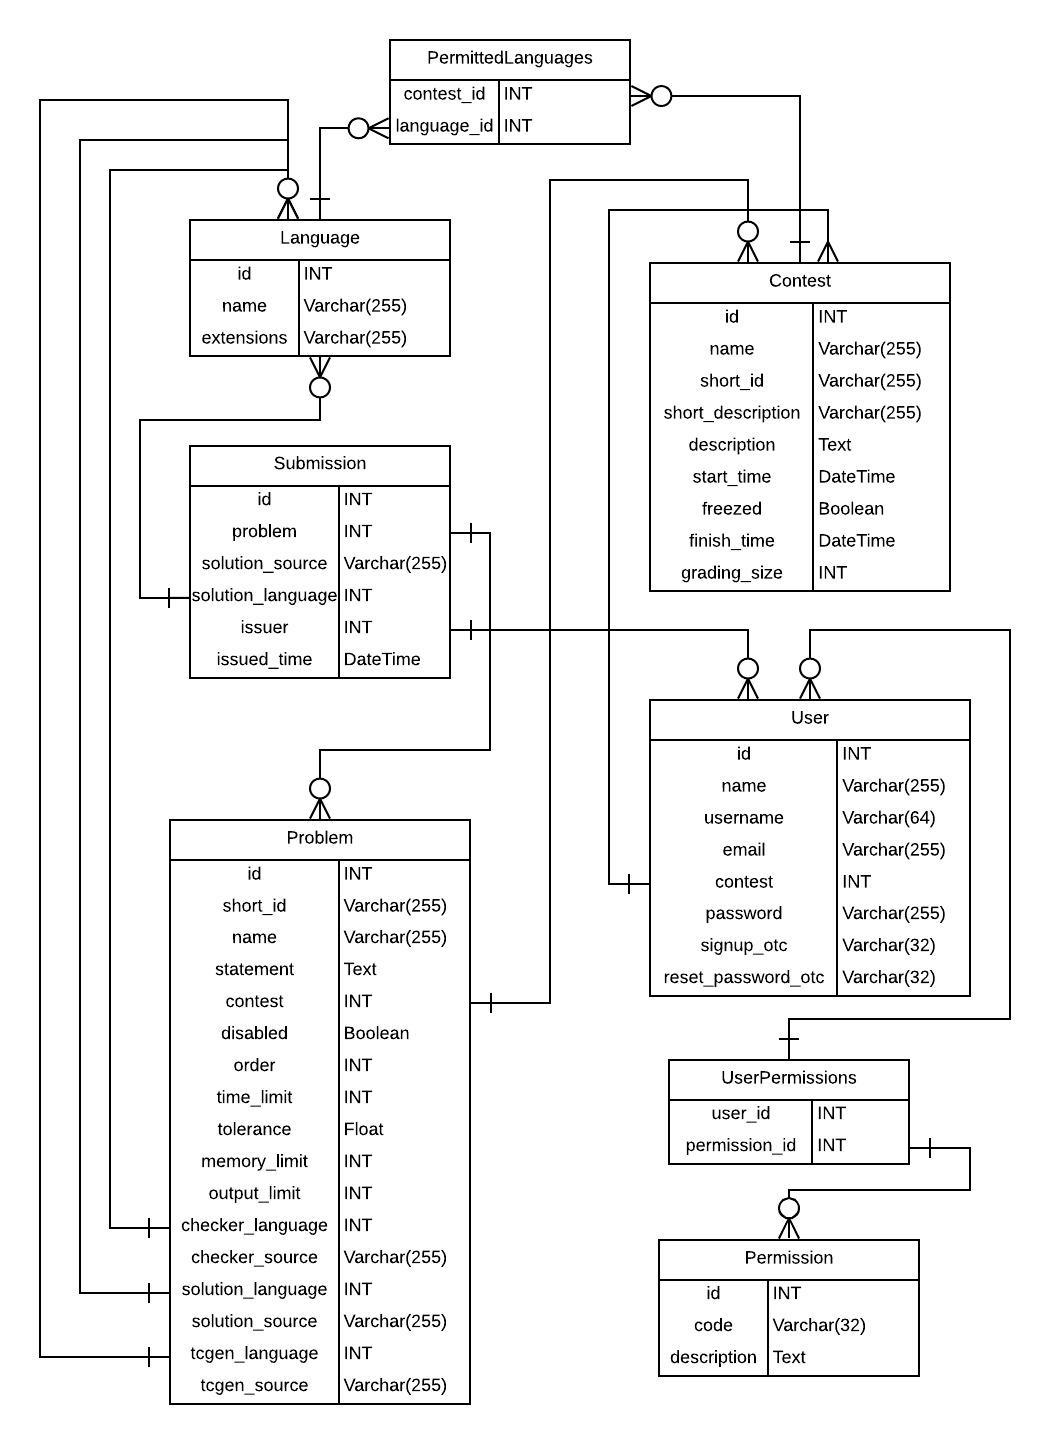
\includegraphics[width=0.8\textwidth]{images/dbschemas}
    \caption{Skema Basis Data Sistem Manajemen Kompetisi}
    \label{fig:dbschemas}
\end{figure}

\par Dalam menjalankan fungsinya, \textit{UGServer} menggunakan sistem manajemen basis data untuk menyimpan informasi terkait kompetisi. Pada saat ini, \textit{UGServer} dapat berjalan menggunakan sistem basis data \textit{Postgresql} atau \textit{SQLite}. \textit{Framework django} memiliki fitur \textit{ORM} yang siap digunakan untuk basis data yang bersifat relasional. Karena adanya fitur tersebut, data lebih mudah untuk diatur menggunakan basis data relasional. Oleh karena itu, pada Tugas Akhir ini penyimpanan data dilakukan menggunakan sistem basis data relasional. Gambar \ref{fig:dbschemas} merupakan skema basis data yang digunakan untuk menyimpan informasi terkait kompetisi.

\subsection{Manajemen Pengguna} \label{subsec:user-management}

% akun
\par \textit{UGServer} memberikan layanan untuk melakukan manajemen pengguna. Pengguna pada \textit{UGrade} terikat pada suatu kompetisi. Pengguna pada suatu kompetisi tidak dapat mengikuti kompetisi lain. Pengguna yang ingin mengikuti dua buah kompetisi harus membuat dua akun. Pengguna dapat membuat akun dengan cara membuat kompetisi. Ketika seseorang membuat kompetisi, maka sebuah akun akan tercipta sesuai dengan alamat \textit{email} orang tersebut. Selain itu, akun dapat dibuat dengan mengundang orang lain ke dalam kompetisi.

% otentikasi
\par Akun yang pertama kali dibuat hanya mengandung informasi alamat \textit{email} pengguna dan kode untuk otentikasi. Kode tersebut akan dikirim ke \textit{email} pengguna. Hal ini berfungsi sebagai cara untuk mengotentikasi pengguna dengan cara mengotentikasi \textit{email} pengguna. Pengguna kemudian harus memasukkan kode tersebut untuk mengotentikasi dirinya. Pengguna yang telah terotentikasi akan memasukkan informasi mengenai nama lengkap, \textit{username} dan kata sandi. Nama lengkap merupakan nama yang akan ditampilkan pada antar muka kompetisi. \textit{Username} merupakan nama pengguna yang unik untuk setiap kontes dan bersifat mudah untuk dibaca oleh manusia. Setelah melakukan otentikasi \textit{email}, pengguna selanjutnya dapat melakukan otentikasi dengan kombinasi kompetisi yang diikuti, alamat \textit{email} dan kata sandi yang dipilih. 

% emai + username unik untuk setiap kompetisi
\par Setiap pengguna dalam suatu kompetisi memiliki alamat \textit{email} dan \textit{username} yang unik. Dalam dua kompetisi berbeda bisa saja terdapat akun dengan alamat \textit{email} yang sama. Hal ini dikarenakan akun pengguna terikat pada suatu kompetisi sehingga seorang pengguna dapat diidentifikasi dengan menggunakan informasi kompetisi yang diikutinya dan alamat \textit{email} atau \textit{username}-nya.

\begin{figure}[ht!]
    \centering
    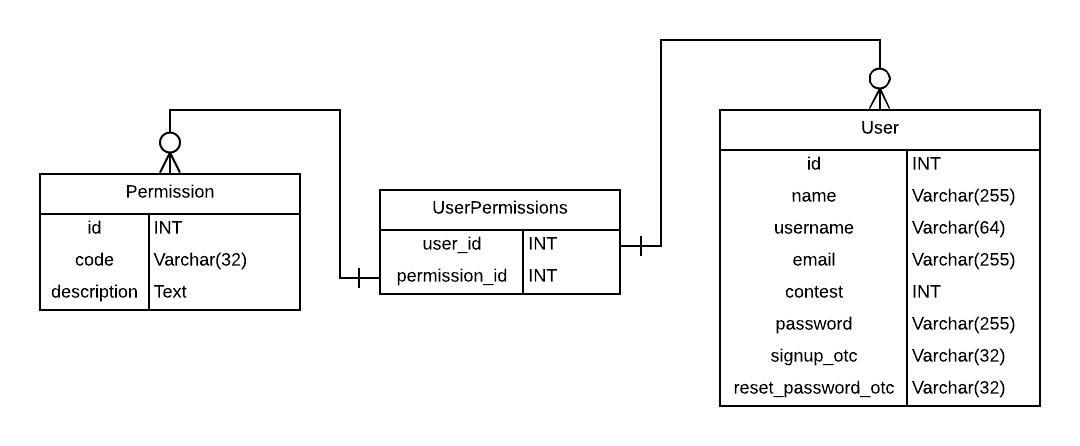
\includegraphics[width=\textwidth]{images/user-schema}
    \caption{Skema Basis Data Sistem Manajemen Pengguna}
    \label{fig:user-schema}
\end{figure}

% user permissions
Pengguna dalam perangkat lunak ini umumnya meliputi juri, peserta dan admin. Perangkat lunak \textit{UGServer} sebenarnya tidak membeda-bedakan pengguna sebagai juri, peserta ataupun admin. Otorisasi dilakukan dengan memberikan label \textit{permission} kepada setiap pengguna yang ada. Setiap pengguna memiliki himpunan \textit{permission} yang menandakan aksi-aksi apa saja yang dapat dilakukan. Pada saati ini, terdapat beberapa \textit{permission} yang mengatur hak akses pengguna yaitu:
\begin{enumerate}
    \item \textit{update:contest}: pengguna dengan \textit{permission} ini dapat mengubah informasi kompetisi.
    \item \textit{create:problems}: pengguna dengan \textit{permission} ini dapat membuat soal baru.
    \item \textit{read:problems}: \textit{permission} ini menandakan seorang pengguna dapat melihat dan membaca soal.
    \item \textit{read:disabledProblems}: beberapa soal dapat ditandai sebagai \textit{disabled} sehingga tidak dapat dibaca oleh pengguna yang tidak memiliki \textit{permission} ini.
    \item \textit{update:problems}: pengguna dengan \textit{permission} ini dapat mengubah informasi soal. Soal yang dapat diubah hanyalah soal yang dapat dilihatnya.
    \item \textit{delete:problems}: sebuah soal dapat dihapus oleh pengguna yang memiliki \textit{permission} ini. Soal yang dapat diubah hanya soal yang dapat dilihat oleh pengguna yang bersangkutan.
    \item \textit{invite:users}: \textit{permission} ini memungkinkan pengguna untuk mengundang pengguna lain.
    \item \textit{update:usersPermissions}: seorang pengguna dapat mengubah \textit{permission} dari pengguna lain jika memiliki \textit{permission} ini.
    \item \textit{delete:users}: pengguna dapat menghapus keanggotaan pengguna lain jika memiliki \textit{permission} ini.
    \item \textit{read:submissions}: dengan \textit{permission} ini, pengguna dapat melihat semua jawaban pengguna lain. \textit{Permission} ini biasanya diberikan untuk juri.
    \item \textit{create:submissions}: \textit{permission} ini memungkinkan pengguna untuk mengirimkan jawabannya. Pengguna tanpa \textit{permission} ini dapat dipandang sebagai seorang penonton.
\end{enumerate}
Pemberian \textit{permission} untuk setiap pengguna bertujuan untuk meningkatkan \textit{granularitas} pada hak akses untuk setiap pengguna. Gambar \ref{fig:user-schema} merupakan skema basis data yang digunakan untuk melakukan manajemen pengguna.

% TODO: jelasin API

\subsection{Manajemen Soal}

\begin{figure}[ht!]
    \centering
    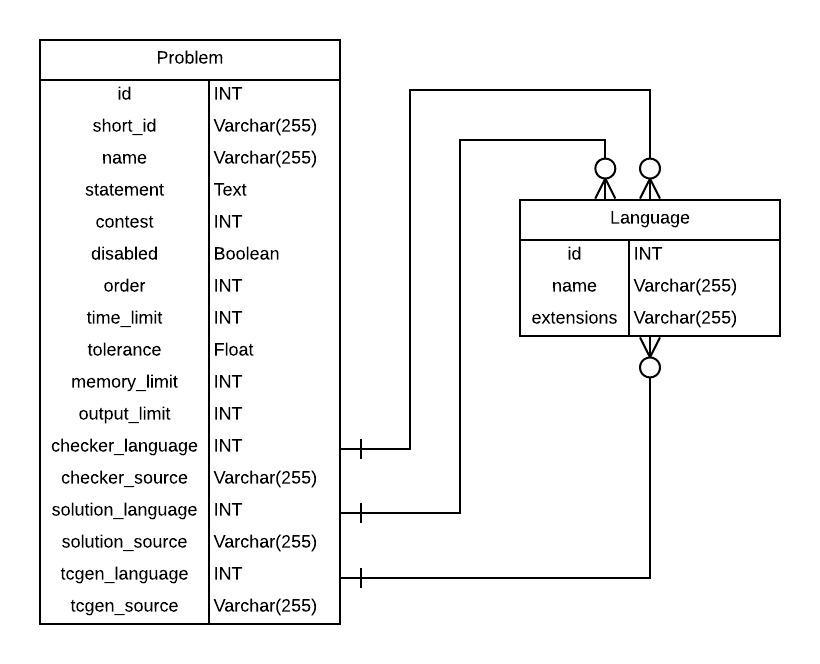
\includegraphics[width=0.8\textwidth]{images/problem-schema}
    \caption{Skema Basis Data Sistem Manajemen Soal}
    \label{fig:problem-schema}
\end{figure}

\par Setiap soal pada \textit{UGServer} akan terikat pada suatu kompetisi. Suatu soal tidak dapat berada pada dua kompetisi sekaligus. Jika terdapat soal yang sama pada kompetisi yang berbeda, maka soal tersebut harus ditambahkan dua kali dan tetap dianggap soal yang berbeda. Setiap soal pada kompetisi memiliki nama dan \textit{short id}. Nama soal merupakan judul soal yang akan ditampilkan pada sistem antar muka yang digunakan pengguna. \textit{Short id} merupakan kode soal yang unik untuk setiap kompetisi dan mudah untuk dibaca oleh manusia. \textit{Short id} berguna untuk mengidentifikasi soal dengan mudah.

\par Informasi mengenai soal disimpan di sistem basis data pada tabel \textit{problems}. Skema basis data yang digunakan untuk menyimpan informasi soal digambarkan pada Gambar \ref{fig:problem-schema}. Aksi-aksi yang dapat dilakukan oleh pengguna terhadap soal ditentukan berdasarkan \textit{permission} yang dimiliki oleh pengguna tersebut.

% TODO: screenshot ui

\par Setiap soal memiliki deskripsi soal. Deskripsi soal merupakan penjelasan mengenai soal, format masukan, format keluaran, contoh masukan dan contoh keluaran. Deskripsi soal ditulis dalam format \textit{markdown} dan disimpan pada \textit{field} \textit{statement} pada tabel \textit{problems}. Pemilihan format \textit{markdown} bertujuan untuk kemudahan melakukan penyimpanan deskripsi soal. Beberapa sistem \textit{online judge} lain memungkinkan melakukan penyimpanan soal dalam bentuk \textit{file} seperti \textit{pdf}. \textit{UGServer} tidak mendukung penyisipan \textit{file} pada deskripsi soal. Hal ini bertujuan untuk memudahkan implementasi.

\par Untuk melakukan penilaian terhadap jawaban peserta, setiap soal dilengkapi dengan beberapa informasi terkait penilaian. Beberapa informasi yang terkait dengan penilaian adalah: batas waktu eksekusi, batas penggunaan \textit{memory}, batas \textit{output file} yang dihasilkan, faktor toleransi, \textit{testcase generator}, solusi juri dan \textit{checker}. Batas waktu eksekusi disimpan pada \textit{field timelimit} dalam bentuk bilangan bulat yang menyatakan lamanya batas waktu eksekusi dalam satuan milidetik. Batas waktu ini digunakan oleh \textit{autograder} untuk menghentikan program secara paksa ketika berjalan terlalu lama. Batas penggunaan memory dan \textit{output file} yang dihasilkan disimpan pada \textit{field memorylimit} dan \textit{outputlimit} di tabel \textit{problems}. Batas tersebut disimpan dalam bentuk bilangan bulat yang menyatakan batas dalam satuan \textit{bytes}. Faktor toleransi disimpan pada \textit{field tolerance} di tabel \textit{problems} sebagai \textit{float}.

\par Dalam melakukan penilaian, \textit{autograder} memerlukan informasi mengenai \textit{testcase generator}, solusi juri, dan \textit{checker}. Informasi tersebut berupa \textit{source code} pada bahasa pemrograman tertentu. \textit{UGServer} menyimpan informasi bahasa pemrograman yang digunakan oleh \textit{testcase generator}, solusi juri dan \textit{checker} pada sistem basis data sebagai \textit{foreign key} ke tabel \textit{languages}. Informasi bahasa pemrograman tersebut disimpan pada \textit{field tcgen\_language, solution\_language}, dan \textit{checker\_language} di tabel \textit{problems}. Informasi mengenai kode sumber tidak disimpan dalam sistem basis data karena dianggap kurang efisien jika ukuran \textit{source code} terlalu besar. Oleh karena itu, kode sumber disimpan sebagai \textit{file} yang berada pada \textit{disk}. Dengan begitu, sistem basis data hanya perlu menyimpan informasi mengenai alamat file dari \textit{source code} yang disimpan.

% TODO: graphql API

\par Pengguna dapat melakukan beberapa aksi pada soal yang ada pada sistem seperti: melihat daftar soal, membaca soal, menambah soal, mengubah soal, dan menghapus soal. Pengguna hanya dapat melakukan aksi-aksi tersebut sesuai izin yang dimilikinya seperti yang sudah dijelaskan pada bagian \ref{subsec:user-management}. Aksi-aksi tersebut dapat dilakukan menggunakan \textit{GraphQL API}.

\subsection{Manajemen Jawaban}

\par Peserta maupun juri dapat mengirimkan jawabannya terhadap suatu soal jika memiliki \textit{permission create:submissions}. Jawaban terhadap suatu soal berupa \textit{source code} yang ditulis pengguna dalam bahasa pemrograman tertentu yang diizinkan. Pada saat ini, bahasa pemrograman yang dapat digunakan adalah C dan C++. Pengguna dapat mengirimkan jawaban melalui \textit{GraphQL API}.

\begin{figure}[ht!]
    \centering
    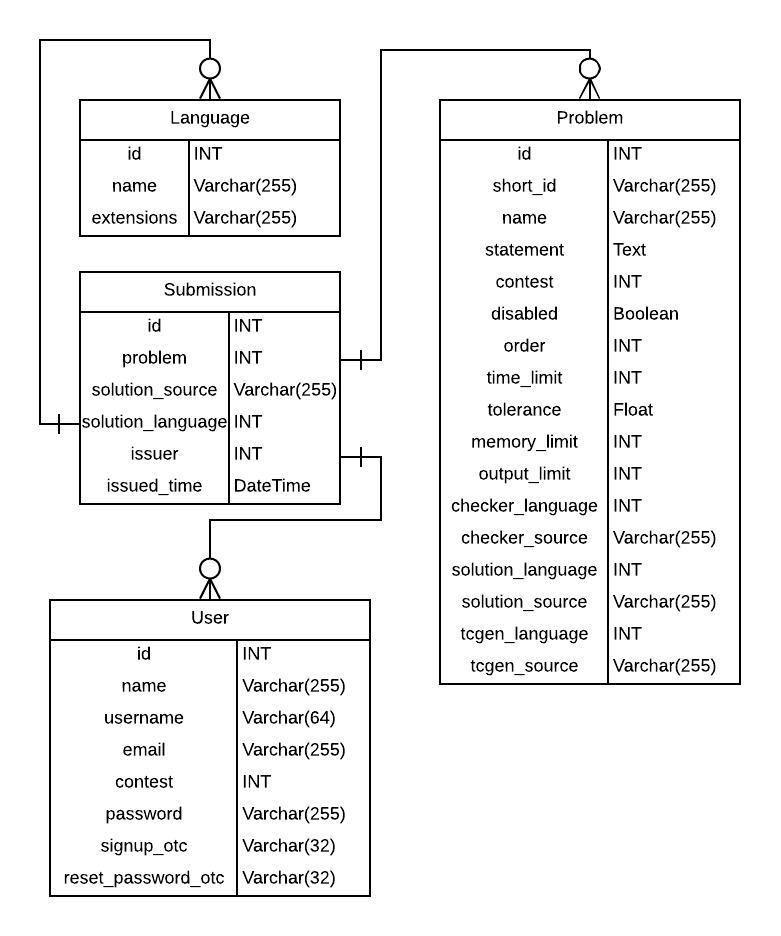
\includegraphics[width=0.8\textwidth]{images/submission-schema}
    \caption{Skema Basis Data Sistem Manajemen Jawaban}
    \label{fig:submission-schema}
\end{figure}

\par \textit{Source code} dari jawaban dari pengguna akan disimpan dalam bentuk \textit{file} yang berada pada \textit{disk}. Selain \textit{source code}, terdapat informasi lain pada jawaban pengguna yang disimpan seperti bahasa pemrograman yang digunakan, waktu pengiriman jawaban, pengirim jawaban dan soal yang bersangkutan. Informasi tersebut disimpan dalam basis data pada tabel \textit{submission}. Gambar \ref{fig:submission-schema} merupakan skema basis data yang digunakan untuk menyimpan jawaban.

\par Setiap jawaban yang berhasil dikirim oleh pengguna akan dinilai oleh \textit{grader}. \textit{Grader} akan berjalan secara otomatis ketika jawaban peserta disimpan. \textit{Grader} kemudian akan menentukan \textit{verdict} dari jawaban peserta. \textit{Verdict} merupakan hasil penilaian terhadap jawaban peserta. Jenis \textit{verdict} yang digunakan adalah:
\begin{enumerate}
    \item \textit{Accpeted}: menandakan bahwa jawaban memberikan keluaran yang benar dan memenuhi batasan.
    \item \textit{Wrong Answer}: menandakan bahwa jawaban memberikan keluaran yang salah tetapi memenuhi batasan.
    \item \textit{Memory Limit Exceeded}: menandakan bahwa jawaban menggunakan terlalu banyak \textit{memory} melebihi batasan yang ditetapkan.
    \item \textit{Time Limit Exceeded}: menandakan bahwa jawaban melebihi batasan waktu yang sudah ditetapkan.
    \item \textit{Runtime Error}: menandakan bahwa jawaban tidak berhasil dieksekusi karena adanya kesalahan pada jawaban.
    \item \textit{Compile Error}: menandakan jawaban tidak dapat dikompilasi.
    \item \textit{Internal Error}: menandakan adanya kesalahan pada sistem \textit{UGrade} sehingga jawaban tidak dapat dinilai.
\end{enumerate}

\subsection{Penilain Jawaban}

\par Setiap jawaban yang dikirimkan oleh pengguna akan dinilai secara otomatis oleh \textit{UGServer}. Penilaian dilakukan secara \textit{asynchronous}. Oleh karena itu, peserta tidak perlu menunggu penilaian selesai untuk melakukan aksi-aksi lain. Seringkali terdapat beberapa masalah teknis yang mengakibatkan jawaban peserta perlu dinilai ulang. Oleh sebab itu, setiap jawaban peserta dapat dinilai lebih dari satu kali. Hasil penilaian yang digunakan adalah hasil penilaian yang terakhir.

\subsubsection{\textit{Grading Group}}

\par Penilaian pada sebuah jawaban disebut sebagai \textit{grading group}. Setiap jawaban dapat dinilai lebih dari satu kali dan memiliki lebih dari satu \textit{grading group}. Adanya \textit{grading group} berguna untuk melakukan penilaian terhadap jawaban peserta lebih dari satu kali. Jika terdapat perubahan \textit{testcase} atau perubahan batasan waktu pada suatu soal, maka perlu adanya penilaian ulang. Penilaian ulang dapat dilakukan dengan membuat \textit{grading group} baru untuk setiap penilaian.

\begin{figure}[ht!]
    \centering
    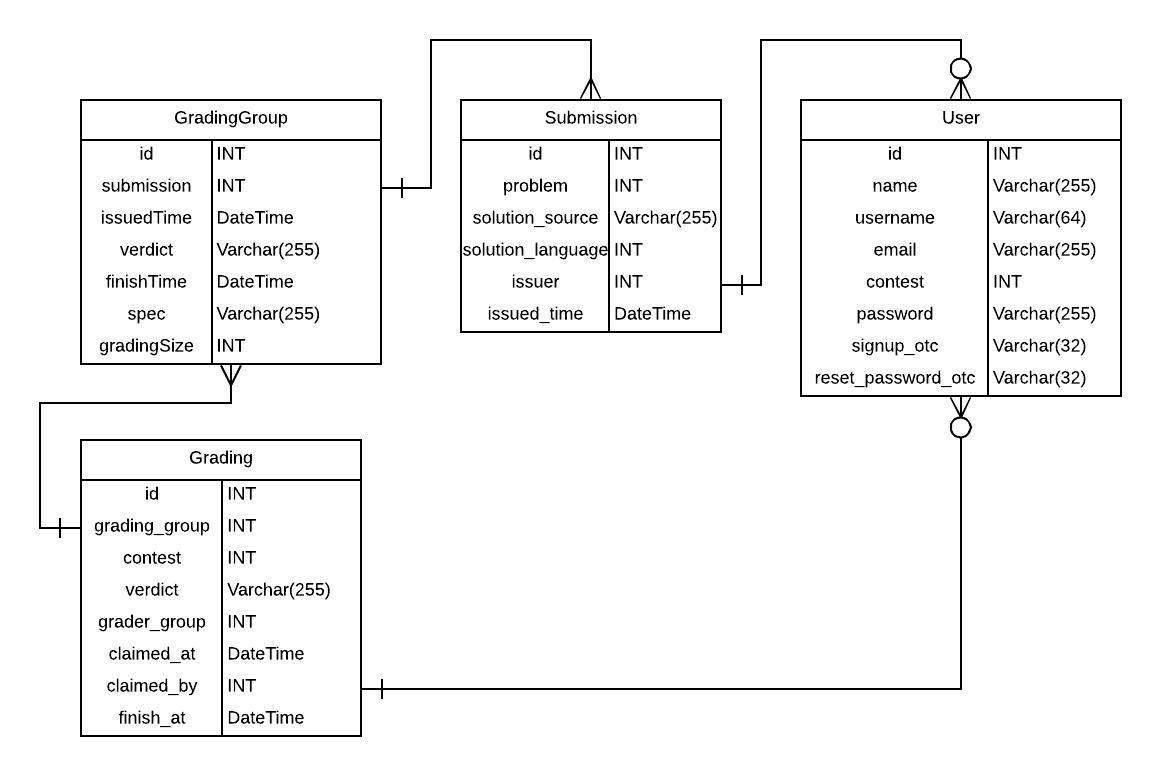
\includegraphics[width=\textwidth]{images/grader-schema}
    \caption{Skema Penilaian Jawaban Pengguna}
    \label{fig:grader-schema}
\end{figure}

\par Informasi dari \textit{grading group} disimpan dalam tabel \textit{GradingGroups} pada sistem basis data. Setiap \textit{grading group} memiliki informasi mengenai jawaban peserta, catatan waktu terciptanya \textit{grading group}, \textit{verdict}, spesifikasi penilaian, catatan waktu selesainya penilaian, dan \textit{grading size}. Informasi-informasi tersebut disimpan sebagai \textit{field} dalam tabel \textit{GradingGroups}. Spesifikasi penilaian berupa \textit{archive file} dan disimpan sebagai \textit{file} dalam \textit{disk}. Field \textit{spec} pada tabel \textit{GradingGroups} menyimpan informasi alamat \textit{file} dari spesifikasi penilaian. Skema basis data yang digunakan untuk melakukan penilaian ditunjukkan pada Gambar \ref{fig:grader-schema}.

\par Penilaian diawali dengan pembuatan spesifikasi penilaian. Spesifikasi penilaian berisi informasi mengenai \textit{testcase generator}, solusi juri, \textit{checker}, solusi peserta dan batasan soal. Informasi tersebut disimpan sebagai \textit{file} dengan format \textit{tar}. Spesifikasi penilain tersebut terdiri dari beberapa file sebagai berikut:
\begin{enumerate}
    \item tcgen.cpp\\ merupakan kode sumber \textit{testcase generator} dari soal. Ekstensi dari \textit{file} dapat berbeda sesuai bahasa pemrograman yang digunakan.
    \item solution.cpp\\ merupakan kode sumber  solusi juri pada soal yang bersangkutan. Ekstensi dari \textit{file} dapat berbeda sesuai bahasa pemrograman yang digunakan.
    \item checker.cpp\\ merupakan kode sumber \textit{checker} dari soal. Ekstensi dari \textit{file} dapat berbeda sesuai dengan bahasa pemrograman yang digunakan.
    \item submission.cpp\\ merupakan kode sumber solusi peserta. Ekstensi dari \textit{file} dapat berbeda sesuai dengan bahasa pemrograman yang digunakan.
    \item lang.json\\ \textit{file} ini berisi \textit{JSON document} yang menjelaskan bahasa pemrograman yang digunakan sebagai \textit{testcase generator}, solusi juri, \textit{checker} dan solusi peserta. \textit{JSON document} pada \textit{file} ini hanya berisi empat \textit{key} yaitu \textit{tcgen}, \textit{solution}, \textit{checker}, dan \textit{submission}. Setiap \textit{key} pada \textit{file} ini memiliki \textit{value} yaitu bahasa \textit{ID} dari bahasa pemrograman yang digunakan.
    \item problem.json\\ \textit{file} ini berisi \textit{JSON document} yang menjelaskan batasan dari soal. \textit{JSON document} pada file ini berisi empat buah \textit{key} yaitu \textit{timeLimit}, \textit{outputLimit}, \textit{memoryLimit}, dan \textit{tolerance}. Setiap \textit{key} pada \textit{file} ini memiliki \textit{value}  berupa bilangan yang menjelaskan batasan dari soal.
\end{enumerate}
\par \textit{File} spesifikasi penilaian ini nantinya akan diunduh oleh \textit{autograder} yang berjalan pada komputer pengguna.

\subsubsection{\textit{Grading Size}}

\par Setiap penilaian yang ditandai dengan \textit{grading group} memiliki suatu nilai \textit{grading size}. Nilai dari \textit{grading size} digunakan untuk mengurangi risiko serangan yang mungkin dilakukan pengguna. Sebuah penilaian dapat dilakukan oleh lebih dari satu \textit{worker}. Setiap worker akan memberikan hasil penilaiannya kepada \textit{UGServer}. Jawaban peserta akan dinilai benar ketika mayoritas dari \textit{worker} yang melakukan penilaian memberikan \textit{verdict} \textit{accepted}. Nilai dari \textit{grading size} mengindikasikan banyaknya \textit{worker} yang melakukan penilaian.

\par Nilai \textit{grading size} yang besar akan lebih aman karena dapat lebih mengurangi risiko kecurangan peserta. Hal ini dikarenakan kemungkinan terjadinya kecurangan lebih kecil sebab \textit{worker} yang bekerja lebih banyak. Meskipun begitu, tingginya nilai \textit{grading size} menyebabkan proses penilaian menjadi lebih lambat karena penilaian harus menunggu banyak \textit{worker} untuk selesai terlebih dahulu. Sebaliknya, nilai \textit{grading size} yang kecil dapat mempercepat penilaian akan tetapi mengurangi keamanan. Nilai \textit{grading size} dapat diatur dalam pengaturan kompetisi oleh pengguna yang memiliki \textit{permission} \textit{update:contests}.

\par Karena setiap jawaban dapat dinilai lebih dari satu kali, perlu ada entitas yang merepresentasikan penilaian sebuah jawaban oleh sebuah \textit{worker}. Entitas tersebut dinamakan \textit{grading}. Sebuah \textit{grading} memiliki informasi mengenai \textit{grading group} terkait, \textit{verdict}, \textit{grader group}, catatan waktu penilaian, dan pengguna yang melakukan penilaian. Informasi ini disimpan di dalam basis data pada tabel \textit{Gradings}.

\par Secara singkat, setiap jawaban dapat memiliki beberapa \textit{grading group} yang merepresentasikan sebuah penilaian terhadap jawaban. Hasil penilaian jawaban pada sebuah \textit{grading group} merupakan hasil penilaian yang dilakukan oleh banyak \textit{worker}. Banyaknya \textit{worker} yang melakukan penilaian adalah sebanyak \textit{grading size}. Setiap penilaian yang dilakukan oleh \textit{worker} direpresentasikan menjadi sebuah \textit{grading}. Secara singkat dapat dikatakan bahwa setiap \textit{grading group} memiliki \textit{grading} sebanyak \textit{grading size}.

\subsubsection{\textit{Grader Group}}

\par Adanya nilai dari \textit{grading size} bertujuan agar setiap jawaban dapat dinilai lebih dari satu \textit{worker}. \textit{Worker} yang melakukan penilaian terhadap suatu jawaban tentunya harus merupakan \textit{worker} yang berbeda. Untuk mengatasi hal ini, setiap \textit{grading} dan \textit{worker} memiliki sebuah nilai \textit{grader group}. \textit{Worker} dengan nilai \textit{grader group} tertentu hanya dapat melakukan penialain terhadap \textit{grading} yang memiliki nilai \textit{grader group} yang sama. Setiap penilaian jawaban peserta, akan dibuat \textit{grading size} buah \textit{grading} yang memiliki nilai \textit{grader group} yang unik yaitu dari nol hingga $\textit{grading size} - 1$. Setiap \textit{worker} dengan \textit{grader group} $K$ hanya akan melakukan penilaian terhadap \textit{grading} yang memiliki nilai \textit{grader group} $K$.

\par Nilai \textit{grader group} dari setiap \textit{worker} dihitung dengan cara melakukan \textit{hash} pada ID \textit{worker}. Setiap \textit{worker} memiliki ID berupa integer yang unik. Nilai \textit{grader group} sebuah worker dihitung dengan formula $\textit{grader\_group} = hash(W_{id}) \bmod \textit{grading\_size}$. Dengan mengasumsikan jumlah \textit{worker} cukup banyak dibandingkan dengan nilai \textit{grading size}, maka cara ini akan mengelompokkan menjadi \textit{grading size} buah kelompok dengan anggota yang kira-kira sama banyak. Cara ini dipilih karena perhitungannya yang cepat, mudah dan dapat mengelompokkan \textit{worker} secara rata.

\begin{figure}[ht!]
    \centering
    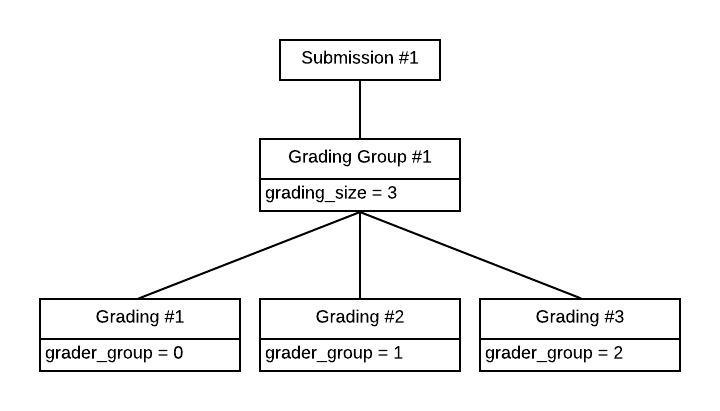
\includegraphics[width=0.6\textwidth]{images/grading-example-1}
    \caption{Contoh Proses Pembuatan \textit{Grading}}
    \label{fig:grading-example-1}
\end{figure}

\par Sebagai contoh, seorang pengguna telah melakukan pengiriman jawaban terhadap suatu soal. Setelah pengiriman jawaban tersebut berhasil dilakukan, akan tercipta sebuah \textit{submission} yang dapat kita beri nama \textit{Submission \#1}. \textit{UGServer} kemudian akan secara otomatis membuat \textit{grading group} untuk menilai jawaban tersebut. Kita dapat memisalkan \textit{grading group} tersebut bernama \textit{Grading Group \#1}. Pada \textit{Grading Group \#1} terdapat informasi mengenai \textit{grading size}. Informasi \textit{grading size} didapatkan dari konfigurasi kompetisi. Pengguna dengan \textit{permission update:contest} dapat mengubah nilai ini. Dalam contoh ini, kita misalnya nilai \textit{grading size} dari kompetisi tersebut adalah tiga. Setelah \textit{grading group} terbentuk, \textit{UGServer} akan membuat \textit{grading size} buah \textit{grading}. Dalam contoh ini berarti akan tercipta tiga buah \textit{grading}. Untuk kemudahan penjelasan, tiga buah \textit{grading} ini dapat kita sebut dengan \textit{Grading \#1} , \textit{Grading \#2}, dan \textit{Grading \#3}. Setiap \textit{grading} yang diciptakan akan memiliki nilai \textit{grader group} yang unik dan terurut dari nol hingga $\textit{grading size} - 1$. Dalam contoh ini \textit{Grading \#1} memiliki nilai \textit{grader group} nol, \textit{Grading \#2} memiliki nilai \textit{grader group} satu, dan \textit{Grading \#3} memiliki nilai \textit{grader group} dua. Gambar \ref{fig:grading-example-1} menggambarkan \textit{submission}, \textit{grading group} dan \textit{grading} pada contoh di paragraf ini.

\begin{figure}[ht!]
    \centering
    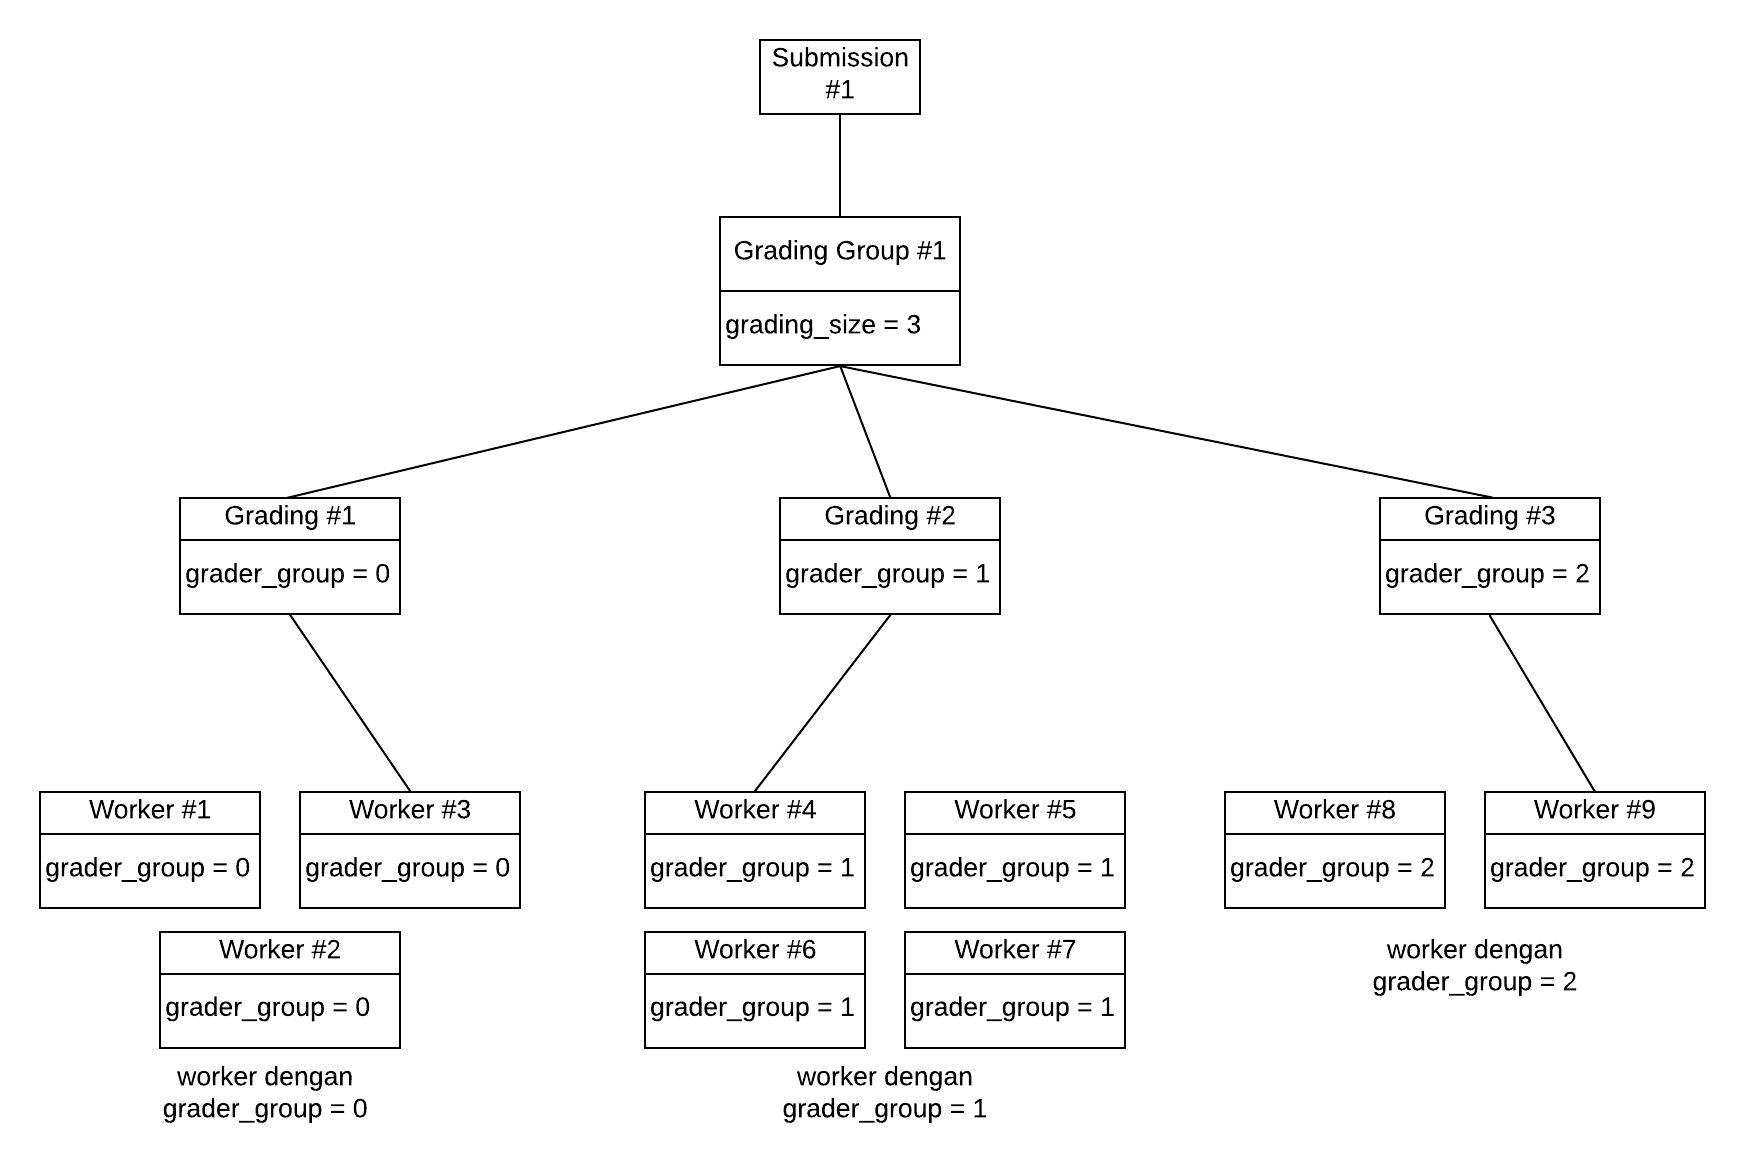
\includegraphics[width=\textwidth]{images/grading-example-2}
    \caption{Contoh Proses Penilaian Oleh \textit{Worker}}
    \label{fig:grading-example-2}
\end{figure}

\par Setelah terbentuk tiga buah \textit{grading} seperti pada paragraf sebelumnya, penilaian dapat mulai dilakukan oleh \textit{worker}. \textit{Worker} secara periodik akan selalu bertanya pada \textit{UGServer} apakah terdapat \textit{grading} yang perlu dikerjakan. \textit{UGServer} akan memberikan \textit{grading} yang sesuai dengan nilai dari \textit{grader group} \textit{worker} yang bersangkutan. Setiap \textit{grading} memiliki informasi \textit{claimed\_by} yang akan berisi ID dari peserta yang sedang melakukan penilaian terhadap \textit{grading} tersebut. Nilai tersebut bertujuan agar \textit{grading} yang sedang dinilai tidak akan dinilai oleh \textit{worker} lain. Gambar \ref{fig:grading-example-2} menjelaskan pemberian \textit{grading} pada \textit{worker} yang dilakukan oleh \textit{UGServer}.

\par \textit{Worker} yang telah melakukan penilaian akan mengirimkan hasil penilaiannya kepada \textit{UGServer}. \textit{UGServer} kemudian akan mengubah nilai \textit{verdict} dari \textit{grading} dan mencatat waktu selesainya penilaian. Jika jumlah \textit{grading} yang selesai dinilai sudah lebih dari setengah dari \textit{grading size}, maka \textit{verdict} dari \textit{grading group} akan diubah. Setelah tahap tersebut, pengguna dapat melihat hasil akhir penilaiannya. 

% TODO: jelasin API waktu grading

% TODO: use more clear term for worker, grading group, grading size, grading, grader group.

% TODO: tambah kode assign grader group

% TODO: further works

\section{\textit{UGSbox}}

% TODO: jelasin kodenya

\par Dalam menjalankan penilaian, \textit{UGSbox} berperan dalam memberikan isolasi terhadap program-program yang berjalan di komputer pengguna. Program-program yang berjalan pada saat penilaian antara lain adalah: \textit{compiler}, \textit{testcase generator}, solusi peserta, solusi juri, dan \textit{checker}. Program-program ini dapat berisi kode yang membahayakan komputer pengguna yang menjalankannya. Oleh karena itu, diperlukan adanya sistem yang dapat mengisolasi program tersebut sehingga tidak membahayakan komputer pengguna. Pada Tugas Akhir ini, \textit{UGSbox} berperan dalam memberikan isolasi tersebut.

\par \textit{UGSbox} memberikan isolasi pada proses yang berjalan dengan menggunakan beberapa fitur dari linux. Isolasi yang diberikan \textit{ugsbox} antara lain adalah sebagai berikut:
\begin{itemize}
    \item isolasi \textit{filesystem}. \\ Isolasi terhadap \textit{filesystem} dilakukan dengan menggunakan \textit{system call chroot}. Dengan menggunakan \textit{chroot}, direktori \textit{root} dari suatu  proses dapat diganti menjadi direktori lain. Mengganti \textit{root} dari proses mengakibatkan proses tersebut tidak dapat mengakses \textit{file} yang ada di luar \textit{root}. \textit{Filesystem} yang akan digunakan oleh proses dapat dimuat dari \textit{file} yang memiliki format \textit{.tar.xz}. File tersebut dinamakan \textit{image file}. Proses isolasi \textit{filesystem} dimulai dengan melakukan ekstraksi \textit{image file} kemudian mengganti \textit{root} dari proses ke dalam direktori \textit{image file} yang sudah berhasil diekstrak. 

    \item \textit{filesystem binding}. \\ \textit{UGSbox} memberikan fitur \textit{filesystem binding} yang dapat digunakan oleh pengguna untuk memasukkan \textit{filesystem} lain ke dalam \textit{filesystem} yang sudah diisolasi. Fitur ini berguna untuk menyimpan \textit{testcase} ke dalam suatu \textit{filesystem} khusus yang kemudian dapat dimuat ke dalam \textit{filesystem} yang sudah diisolasi.

    \item isolasi \textit{network}. \\ Untuk menjaga keamanan, setiap proses yang berjalan di dalam lingkungan yang diisolasi tidak boleh menggunakan \textit{network} untuk berkomunikasi dengan dunia luar. Untuk mengatasi masalah ini, \textit{UGSbox} menggunakan fitur \textit{namespace} dari linux. Proses yang diisolasi akan mendapat \textit{namespace} dengan \textit{network interface} yang terisolasi dari \textit{network interface} milik \textit{host}.

    \item isolasi \textit{user}. \\ Selain isolasi \textit{network}, \textit{namespace} pada Linux juga digunakan untuk melakukan isolasi \textit{user}. Dengan mengisolasi \textit{user}, proses yang terisolasi tidak dapat mengetahui adanya \textit{user} lain di luar lingkungannya.

    \item batas penggunaan CPU dan \textit{memory}. \\ Penggunaan CPU dan \textit{memory} dari proses yang diisolasi tentunya perlu dibatasi. Hal ini bertujuan agar proses yang berjalan tidak memberatkan komputer pengguna ketika penilaian sedang berlangsung. Untuk mengatasi masalah ini, \textit{UGSbox} menggunakan fitur \textit{cgroup} dari linux. Dengan menggunakan \textit{cgroup}, penggunaan \textit{memory} dan CPU dapat dibatasi dan dimonitor. Proses yang menggunakan CPU atau \textit{memory} melebihi batasan akan dihentikan secara paksa. 

    \item batas ukuran \textit{file} yang dapat dihasilkan. \\ Program yang dikirimkan oleh pengguna mungkin saja memuat kode yang dapat memberatkan \textit{disk} karena melakukan penulisan secara terus menerus. Hal ini dapat mengakibatkan komputer pengguna menjadi lambat karena \textit{disk}-nya tidak dapat digunakan. Untuk mengatasi masalah ini, \textit{UGSbox} membatasi ukuran \textit{file} yang dapat diciptakan oleh proses di dalam lingkungan yang diisolasi. Pembatasan ini dicapai dengan menggunakan \textit{system call setrlimit}.

    \item batas jumlah \textit{file} yang dapat dibuka. \\ Untuk meningkatkan keamanan, jumlah \textit{file} yang dapat dibuka oleh proses yang diisolasi juga dibatasi menggunakan \textit{system call setrlimit}.

    \item batas proses yang dapat diciptakan. \\ Selain membatasi ukuran \textit{file} yang dihasilkan, dan jumlah \textit{file} yang dapat dibuka, \textit{UGSbox} juga menggunakan \textit{setrlimit} untuk membatasi proses yang dapat diciptakan.

\end{itemize}

\begin{lstlisting}[caption={Contoh Hasil Eksekusi Perintah \textit{ugsbox}},label={lst:ugsbox-guard},language=Bash,style=BashStyle]
$ ugsbox guard --help
Usage:
  ugsbox guard [flags]

Flags:
  -b, --bind strings               bind host directory to sandbox directory with format <hostdir>:<sandboxdir>. Warning: file owner of binded directory will be changed
  -f, --file-size uint             generated file size limit
  -h, --help                       help for guard
  -i, --image string               compressed sandbox image (in .tar.xz) path
  -m, --memory-limit uint          memory limit in bytes (default 67108864)
  -M, --memory-throttle uint       memory throttle in bytes (default 268435456)
  -n, --nproc uint                 limit process creation e.g.: fork/exec
  -o, --open-file uint             open file limit
  -s, --stack-size uint            limit stack size in bytes
  -E, --stderr string              path (relative to sandbox) to file to be used as stderr
  -I, --stdin string               path (relative to sandbox) to file to be used as stdin
  -O, --stdout string              path (relative to sandbox) to file to be used as stdout
  -t, --time-limit uint            time limit in milisecond (default 10000)
  -T, --walltime-limit uint        wall clock time limit in milisecond (default 10000)
  -w, --working-directory string   working directory of process (default "/home")

Global Flags:
      --debug   show debug log
      --trace   show trace log
\end{lstlisting}

\par \textit{UGSBox} dapat digunakan dengan dua cara yaitu: sebagai \textit{executable program} atau sebagai \textit{library}. Pengguna dapat menggunakan perintah \textit{ugsbox guard} untuk menjalankan \textit{UGSbox} melalui CLI. Kode \ref{lst:ugsbox-guard} merupakan contoh hasil pemanggilan \textit{ugsbox guard}.

\par Selain melalui CLI, \textit{UGSbox} juga dapat digunakan melalui pemanggilan fungsi pada bahasa pemrograman GO. Untuk dapat menggunakan \textit{UGSbox} sebagai \textit{library}, pengguna dapat meng-\textit{import} \textit{package https://github.com/jauhararifin/ugrade} dan \textit{https://github.com/jauhararifin/ugrade/sandbox}. Penggunaan \textit{library} tersebut dapat dapat dilihat pada dokumentasi \textit{UGrade} di \textit{https://godoc.org/github.com/jauhararifin/ugrade}.

\section{\textit{UGJob}}

% TODO: jelasin kodenya

\par \textit{UGJob} merupakan implementasi dari \textit{worker} pada keluarga perangkat lunak \textit{UGrade}. \textit{UGJob} dikembangkan menggunakan bahasa GO dan berperan dalam menilai jawaban pengguna. \textit{UGJob} dikembangkan sebagai sebuah \textit{executable} yang dapat dijalankan melalui CLI. \textit{UGDesktop} akan secara periodik menjalankan \textit{UGJob} untuk melakukan penilaian.

\par Setiap \textit{grading} yang dihasilkan oleh \textit{UGServer} akan dinilai oleh \textit{worker} yang ada pada komputer pengguna. \textit{Worker} pada komputer pengguna tidak perlu mengetahui adanya konsep \textit{grading group}, \textit{grading size}, dan \textit{grader group}. \textit{Worker} hanya perlu meminta \textit{grading} pada \textit{UGServer} untuk dinilai. Dalam meminta \textit{grading}, \textit{worker} hanya perlu mengirimkan ID dari pengguna yang bertindak sebagai \textit{worker}. \textit{UGServer} akan memberikan \textit{grading} yang sesuai dengan ID pengguna dari \textit{worker} tersebut.

\par Di sisi \textit{worker}, semua \textit{grading} yang perlu dinilai akan dipandang sebagai sebuah \textit{job}. Pada Tugas Akhir ini, \textit{job} dapat disamakan dengan \textit{grading} karena sebuah \textit{grading} akan dianggap sebagai sebuah \textit{job} oleh \textit{worker}. Istilah \textit{job} digunakan untuk meningkatkan abstraksi dari \textit{worker}. \textit{Worker} tidak perlu mengetahui konsep penilaian yang dilakukan di sisi \textit{UGServer}. \textit{Worker} tidak perlu mengetahui adanya konsep \textit{grading} pada \textit{UGServer}. Semua penilaian yang perlu dilakukan oleh \textit{worker} akan dianggap sebagai sebuah \textit{job}. Dengan menggunakan istilah \textit{job}, sistem penilaian yang ada pada sisi \textit{UGServer} dapat dengan mudah dimodifikasi tanpa memengaruhi \textit{worker}.

\begin{lstlisting}[caption={Contoh Hasil Eksekusi Perintah \textit{ugjob consume}},label={lst:ugjob-consume},language=Bash,style=BashStyle]
$ ugjob consume --help
This program fetch job from server, execute it and send the result back to server.

Usage:
  ugjob consume [flags]

Flags:
  -h, --help                help for consume
  -u, --server-url string   Server url (default "http://localhost:8000")
  -t, --token string        Your session token

Global Flags:
      --debug   show debug message
      --trace   show trace message
\end{lstlisting}

\par \textit{UGJob} dapat dijalankan melalui CLI dengan mengetikkan perintah \textit{ugjob consume}. \textit{UGJob} memerlukan \textit{token} yang bisa didapatkan oleh pengguna pada saat melakukan \textit{sign in}. \textit{Token} ini berguna untuk mengidentifikasi ID dari pengguna. \textit{UGServer} akan menggunakan \textit{token} untuk menentukan \textit{job} mana yang akan dikerjakan oleh \textit{worker}. Kode \ref{lst:ugjob-consume} merupakan contoh hasil pemanggilan \textit{ugjob consume}.

\par Pemanggilan \textit{ugjob consume} akan menjalankan \textit{worker} pada komputer pengguna dan proses penilaian akan mulai dilakukan. Penilaian diawali dengan pengambilan \textit{job} oleh \textit{UGJob}. \textit{UGJob} akan meminta \textit{job} kepada \textit{UGServer} dengan mengirimkan \textit{GET HTTP request} ke \textit{UGServer} dengan menyertakan \textit{token} yang dimilikinya. \textit{HTTP Request} tersebut akan dikirimkan ke URL \textit{/gradings} pada \textit{UGServer} dengan menyertakan \textit{token} pada bagian \textit{header}.

\par Setiap permintaan \textit{job} yang dilakukan oleh \textit{UGJob} akan diproses oleh \textit{UGServer}. \textit{UGServer} akan memberikan job yang sesuai kepada \textit{UGJob}. Pemberian \textit{job} dilakukan dengan memandang \textit{token} yang disertakan oleh \textit{UGJob} ketika melakukan permintaan \textit{job}. Jika tidak terdapat \textit{job} yang perlu dikerjakan, maka \textit{UGServer} akan memberikan \textit{HTTP response} dengan status 404. \textit{UGServer} akan memberikan \textit{job} kepada \textit{UGJob} dengan bentuk \textit{tar file} yang dikirimkan melalui \textit{body} pada \textit{HTTP response}. Selain itu, \textit{UGServer} juga menyertakan \textit{job token} pada setiap \textit{job} yang dikirimkan. \textit{Job token} ini berguna untuk membedakan antara satu buah \textit{job} dengan yang lainnya.

\par Setelah mendapatkan \textit{job} dari \textit{UGServer}, \textit{UGJob} akan melakukan penilaian dengan mengekstrak \textit{job} yang didapatkannya. \textit{Job} akan diekstrak pada suatu direktori sementara di \textit{/tmp}. Direktori \textit{/tmp} dipilih karena sistem secara otomatis akan menghapus isi dari direktori ini ketika \textit{booting}. Selain itu, direktori ini juga sudah standar digunakan sebagai tempat penyimpanan \textit{file} yang bersifat sementara. Direktori \textit{Job} yang sudah berhasil dinilai secara otomatis akan dihapus oleh \textit{UGJob}. 

\subsection{Pembangkitan \textit{Testcase}}

\par Untuk melakukan penilaian, diperlukan adanya \textit{testcase}. \textit{Testcase} akan dibangkitkan dengan menggunakan program \textit{testcase generator} yang disertakan pada \textit{file} \textit{job}. \textit{Testcase generator} ini pertama-tama dikompilasi menjadi \textit{executable file} kemudian dijalankan. \textit{Testcase} yang dihasilkan oleh \textit{testcase generator} disimpan pada direktori sementara di dalam \textit{/tmp}.

% TODO: jelasin spesifikasi testcase generator & testcase suite

\par Program \textit{testcase generator} hanya membangkitkan masukan dari \textit{testcase}. Keluaran dari \textit{testcase} dibangkitkan dengan menggunakan solusi juri. Untuk membangkitkan keluaran dari \textit{testcase}, solusi juri dikompilasi kemudian dijalankan dengan memberikan input yang berasal dari \textit{testcase generator}. Keluaran dari solusi juri ini akan digunakan sebagai keluaran dari \textit{testcase}.

\par \textit{Testcase} yang sudah terbentuk disimpan pada suatu direktori tertentu. Direktori yang menjadi tempat penyimpanan \textit{testcase} tidak akan dihapus ketika penilaian sudah selesai dilakukan. Hal ini bertujuan agar proses penilaian \textit{job} selanjutnya tidak perlu melakukan pembangkitan \textit{testcase} lagi.

\subsection{Penghitungan Waktu Dan \textit{Memory} Solusi Juri} 

\par Waktu dan \textit{memory} dari eksekusi solusi juri perlu dihitung untuk menentukan batasan waktu dan \textit{memory} solusi peserta. Waktu dan \textit{memory} eksekusi solusi juri dihitung pada saat pembangkitan \textit{testcase}. Solusi juri diperlukan dalam membangkitkan keluaran dari \textit{testcase}. Pada saat keluaran \textit{testcase} dibangkitkan, lamanya waktu eksekusi dan penggunaan \textit{memory}-nya dihitung dan dicatat.

\par Perhitungan waktu eksekusi dilakukan dengan menggunakan \textit{UGSbox}. Proses yang dijalankan menggunakan \textit{UGSbox} dapat dihitung penggunaan waktu dan \textit{memory}-nya. Jika solusi juri melebihi batas waktu yang ditentukan oleh juri, maka \textit{UGJob} akan memberikan \textit{verdict} \textit{internal error} yang menandakan bahwa penilaian gagal dilakukan. Hal ini dapat terjadi ketika komputer peserta sangat lambat.

\subsection{Eksekusi Solusi Peserta}

\par Setelah \textit{testcase} berhasil dibangkitkan dan batasan untuk peserta sudah berhasil dihitung, solusi peserta akan mulai dijalankan. Seperti program lainnya, solusi peserta dijalankan menggunakan \textit{UGSbox} untuk menghindari penggunaan \textit{resource} yang berlebihan dan menghindari risiko dari adanya serangan yang ada pada program solusi peserta.

\par Sebelum solusi peserta dijalankan, tentunya perlu ada proses kompilasi. Proses kompilasi ini dilakukan dengan cara yang sama untuk mengkompilasi program lain. Pada saat kompilasi, beberapa kegagalan mungkin terjadi seperti: kesalahan \textit{syntax}, penggunaan \textit{memory} terlalu besar, dan proses kompilasi berjalan terlalu lama. Jika terjadi kegagalan pada tahap kompilasi, maka \textit{UGJob} akan memberikan \textit{verdict} \textit{compile error}.

\par Penggunaan CPU dan \textit{memory} dari program solusi peserta dibatasi berdasarkan batasan yang diperoleh ketika menjalankan program solusi juri. Jika solusi peserta menggunakan \textit{memory} melebihi batasan yang sudah dihitung, maka \textit{UGJob} akan memberikan \textit{verdict} \textit{memory limit exceeded}. Selain itu, jika solusi peserta berjalan terlalu lama dan melebihi batasan waktu yang sudah dihitung maka \textit{UGJob} akan memberikan \textit{verdict} \textit{time limit exceeded}. Program solusi peserta mungkin saja melakukan kesalahan yang menyebabkan munculnya \textit{error} seperti pembagian dengan nol, atau mengakses alamat \textit{memory} yang belum dialokasikan. Jika hal ini terjadi, maka \textit{UGJob} akan memberikan \textit{verdict} \textit{runtime error}.

\par Keluaran dari program solusi peserta disimpan pada direktori sementara yang diletakkan pada \textit{/tmp}. Selanjutnya keluaran dari program solusi peserta akan dinilai dengan cara dibandingkan dengan keluaran solusi juri. Setelah penilaian selesai dilakukan, keluaran program solusi peserta sudah tidak digunakan lagi. Oleh sebab itu, keluaran program solusi peserta dihapus setelah penilaian selesai dilakukan.

\subsection{Penilaian Keluaran Solusi Peserta}

\par Keluaran dari program solusi peserta perlu dinilai kebenarannya. Penilaian kebenaran dari program solusi peserta dilakukan dengan cara membandingkannya dengan keluaran solusi juri. \textit{UGJob} membandingkan keluaran program solusi peserta dengan program solusi juri dengan menggunakan \textit{checker}.

\par \textit{Checker} merupakan sebuah program yang dibuat oleh juri dan digunakan untuk menilai kebenaran program solusi peserta. Seperti pada program lainnya, perlu adanya proses kompilasi yang dilakukan pada \textit{checker}. Proses kompilasi \textit{checker} dilakukan dengan cara yang sama seperti kompilasi program lainnya.

\lstinputlisting[caption={Contoh Program \textit{Checker}},label={lst:exact-match-checker},language=C,style=CStyle]{listings/exact-match-checker.c}

\par Setelah \textit{checker} selesai dikompilasi, \textit{checker} akan dijalankan dengan memberikan masukan berupa masukan \textit{testcase}, keluaran program solusi juri dan keluaran program solusi peserta. \textit{Checker} kemudian akan memberikan keluaran berupa kebenaran dari program solusi peserta. Kode \ref{lst:exact-match-checker} merupakan contoh \textit{checker} yang membandingkan kesamaan tiap \textit{byte} dari keluaran solusi peserta dan solusi juri.

\par Program \textit{checker} akan memberikan keluaran berupa \textit{string} yang dapat bernilai \textit{AC} atau \textit{WA}. Keluaran \textit{checker} akan bernilai \textit{AC} jika solusi peserta dianggap benar, dan akan bernilai \textit{WA} jika sebaliknya. \textit{UGJob} kemudian akan mengirimkan \textit{verdict} kepada \textit{UGServer} sesuai dengan hasil penilaian \textit{checker}.

\par Program \textit{checker} yang dibuat oleh juri mungkin saja memiliki kesalahan. Kesalahan tersebut mengakibatkan program \textit{checker} menghasilkan \textit{error}. Selain itu, jika program \textit{checker} juga mungkin menggunakan terlalu banyak \textit{memory} dan menghabiskan terlalu banyak \textit{waktu}. Jika hal ini terjadi, maka program \textit{checker} akan dihentikan dan \textit{UGJob} akan menghasilkan \textit{verdict} \textit{internal error}.

\par Setelah penilaian selesai dilakukan dan \textit{verdict} sudah ditentukan, hasil penilaian akan dikirmkan ke \textit{UGServer}. Hasil penilaian yang dikirimkan berupa \textit{verdict} hasil penilaian. Pengiriman dilakukan melalui \textit{POST HTTP request}. \textit{Job token} disertakan pada \textit{header} dari \textit{HTTP request} sebagai identitas dari \textit{job} yang telah diselesaikan.

\section{\textit{UGDesktop}}

\par Dalam kelompok perangkat lunak \textit{UGrade}, pengguna dapat berinteraksi dengan sistem kompetisi dengan \textit{UGDesktop}. \textit{UGDesktop} memudahkan interaksi pengguna dengan memberikan antar-muka berbasis grafis. Pengguna dapat meng-\textit{install} \textit{UGDesktop} pada komputernya. Pengguna kemudian dapat menjalankan \textit{UGDesktop} sebagai aplikasi \textit{desktop} pada komputernya.

\begin{figure}[ht!]
    \centering
    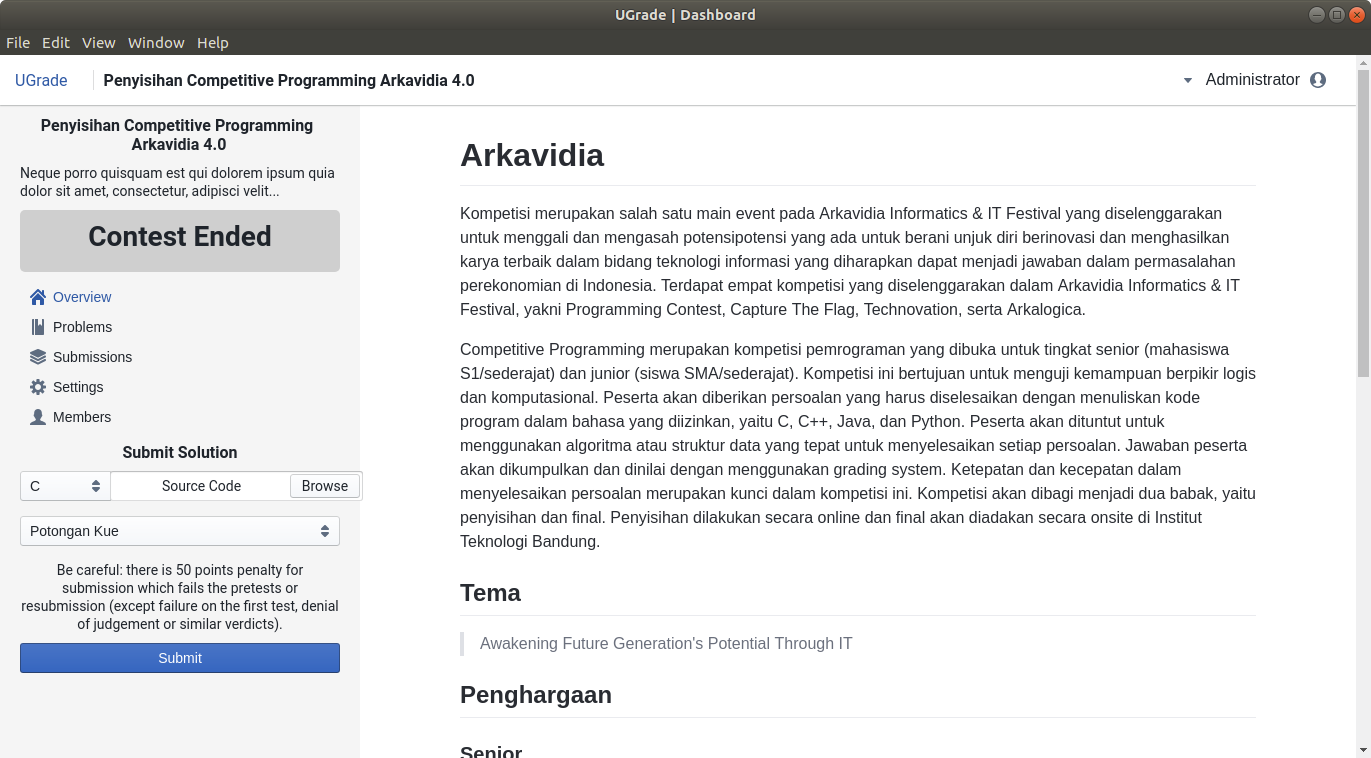
\includegraphics[width=\textwidth]{images/ugdesktop-example}
    \caption{Halaman Kompetisi Dari \textit{UGDesktop}}
    \label{fig:ugdesktop-example}
\end{figure}

\par \textit{UGDesktop} dikembangkan menggunakan \textit{typescript}, \textit{react} dan \textit{electron}. \textit{React} dipilih karena mudah untuk digunakan dan banyak \textit{library} yang mendukung pengembangan aplikasi berbasis \textit{react}. \textit{React} umumnya digunakan untuk mengembangkan aplikasi berbasis \textit{web} dan membutuhkan \textit{web browser} untuk menjalankan aplikasi tersebut. Pengguna membutuhkan aplikasi yang dapat berjalan sebagai \textit{desktop app} untuk dapat menjalankan sistem antar muka pengguna sekaligus \textit{worker}. Untuk mengatasi hal tersebut, \textit{electron} digunakan untuk menjalankan aplikasi \textit{web} yang berbasis \textit{react} sebagai aplikasi \textit{desktop}. Gambar \ref{fig:ugdesktop-example} merupakan contoh salah satu halaman pada \textit{UGDesktop}.

\par Untuk melakukan penilaian, \textit{UGDesktop} secara periodik akan meminta menjalankan \textit{UGJob}. Dalam menjalankan \textit{UGJob}, \textit{UGDesktop} menggunakan \textit{token} yang didapatkannya ketika pengguna melakukan \textit{sign in}. \textit{UGJob} yang dijalankan \textit{UGDesktop} akan meminta \textit{job} dari \textit{UGServer} untuk dinilai.

\section{Pengujian}

\par Pengujian dilakukan dengan menyimulasikan proses pengiriman jawaban oleh pengguna. Sebuah kompetisi diciptakan dengan beberapa pengguna yang akan mengirimkan jawaban secara periodik. Kinerja sistem yang dibangun dibandingkan dengan sistem \textit{online judge} yang bersifat \textit{open source} yaitu \textit{DOMJudge}. \textit{DOMJudge} dipilih karena bersifat \textit{open source} dan sudah populer digunakan untuk menyelenggarakan kompetisi \textit{competitive programming}. \textit{DOMJudge} telah digunakan untuk menyelenggarakan ACM-ICPC, Arkavidia, Vocompfest dan banyak kompetisi lainnya.

\par Selain pengujian kinerja, diperlukan pengujian kebenaran dari sistem yang dibangun. Pengujian kebenaran dilakukan dengan menyimulasikan proses pengiriman jawaban oleh peserta. Kebenaran sistem yang dibangun ditentukan berdasarkan \textit{verdict} penilaian yang diberikan oleh sistem. Sistem yang benar akan memberikan \textit{verdict} yang sama ketika jawaban yang sama dinilai berkali-kali di komputer yang berbeda. Pada pengujian kebenaran, digunakan sebuah soal dengan enam buah jawaban yang diharapkan akan memiliki \textit{verdict} \textit{accepted}, \textit{wrong answer}, \textit{memory limit exceeded}, \textit{time limit exceeded}, \textit{runtime error}, dan \textit{compile error}.

\par Sistem \textit{online judge} yang dibangun perlu memiliki tingkat keamanan yang cukup sehingga tidak membahayakan komputer peserta dan sistem. Pengujian keamanan dilakukan dengan menyimulasikan pengiriman jawaban yang berbahaya ke sistem \textit{online judge}. Jawaban yang dikirimkan adalah sebagai berikut:
\begin{enumerate}
    \item jawaban yang berisi \textit{fork bomb}
    \item jawaban yang berisi \textit{compile bomb}
    \item jawaban yang berisi \textit{reverse shell}
    \item jawaban yang mencoba keluar dari lingkungan \textit{sandbox}
\end{enumerate} 
Komputer yang bertindak sebagai worker diharapkan dapat tetap berjalan setelah jawaban tersebut dieksekusi.

\par Kerahasiaan dan integritas dari \textit{testcase}, solusi juri dan solusi peserta perlu dijaga. Untuk menjaga kerahasiaan dan integritas, diperlukan adanya pengujian. Pengujian integritas dilakukan dengan melakukan percobaan merusak \textit{testcase}, solusi juri dan solusi peserta yang ada pada komputer \textit{worker}. Perusakan pada \textit{testcase}, solusi juri ataupun solusi peserta diharapkan dapat dikenali dan diatasi sehingga hasil penilaian dari \textit{worker} akan tetap benar. Kerahasiaan \textit{testcase}, solusi juri dan solusi peserta hanya akan diuji dengan melihat isi dari \textit{file} \textit{testcase}, solusi juri dan solusi peserta. Kerahasiaan akan dianggap lolos uji jika isi dari \textit{file} \textit{testcase}, solusi juri maupun solusi peserta tidak dapat dibaca oleh pengguna.

% TODO: data pengujian